%	INF219
%	Oskar L. F. Lerivåg
%	3D Printer Tizen-wearable application

\documentclass[a4paper, 12pt]{article}

%Bookmarks
\usepackage[colorlinks=true,urlcolor=cyan,linkcolor=black,citecolor=red,bookmarksopen=true]{hyperref}
\usepackage{bookmark}

\usepackage[utf8]{inputenc}
\usepackage{amsmath}
\usepackage{pgf,tikz}
\usepackage{mathrsfs}
\usepackage{listings}
\usetikzlibrary{arrows}
\usepackage{amssymb}
\usepackage{url}
\usepackage{epigraph}

%Images%
\usepackage{graphicx}
\usepackage{float}

%Margins
\usepackage{geometry}
\geometry{a4paper, margin=3cm}

%Citations
\usepackage[round]{natbib}
\bibliographystyle{plainnat}

\newcommand{\mysection}[1]{\section*{#1} \addcontentsline{toc}{section}{#1}}
\newcommand{\mysubsection}[1]{\subsection*{#1} \addcontentsline{toc}{subsection}{#1}}
\newcommand{\mysubsubsection}[1]{\subsubsection*{#1} \addcontentsline{toc}{subsubsection}{#1}}

\newcommand{\mycitation}[1]{[\citet{#1}]}

\begin{document}

    % % % % % % % % % % % % % % % % %
    %
    %	FORDISE!
    %
    %%%%%%%%%%%%%%%%%%%%%%%%%%%%%%%%%%%%%%%%%
% University Assignment Title Page 
% LaTeX Template
% Version 1.0 (27/12/12)
%
% This template has been downloaded from:
% http://www.LaTeXTemplates.com
%
% Original author:
% WikiBooks (http://en.wikibooks.org/wiki/LaTeX/Title_Creation)
%
% License:
% CC BY-NC-SA 3.0 (http://creativecommons.org/licenses/by-nc-sa/3.0/)
% 
% Instructions for using this template:
% This title page is capable of being compiled as is. This is not useful for 
% including it in another document. To do this, you have two options: 
%
% 1) Copy/paste everything between \begin{document} and \end{document} 
% starting at \begin{titlepage} and paste this into another LaTeX file where you 
% want your title page.
% OR
% 2) Remove everything outside the \begin{titlepage} and \end{titlepage} and 
% move this file to the same directory as the LaTeX file you wish to add it to. 
% Then add \input{./title_page_1.tex} to your LaTeX file where you want your
% title page.
%
%%%%%%%%%%%%%%%%%%%%%%%%%%%%%%%%%%%%%%%%%

%----------------------------------------------------------------------------------------
%	PACKAGES AND OTHER DOCUMENT CONFIGURATIONS
%----------------------------------------------------------------------------------------


\begin{titlepage}


    \newcommand{\HRule}{\rule{\linewidth}{0.5mm}} % Defines a new command for the horizontal lines, change thickness here

    \center % Center everything on the page

    %----------------------------------------------------------------------------------------
    %	HEADING SECTIONS
    %----------------------------------------------------------------------------------------

    \textsc{\LARGE Universitetet i Bergen}\\[1.5cm] % Name of your university/college
    \textsc{\Large INF219}\\[0.5cm] % Major heading such as course name
    \textsc{\large Project in informatics I}\\[0.5cm] % Minor heading such as course title

    %----------------------------------------------------------------------------------------
    %	TITLE SECTION
    %----------------------------------------------------------------------------------------

    \HRule \\[0.4cm]
    { \huge \bfseries 3D Printer Tizen-wearable application}\\[0.4cm] % Title of your document
    \HRule \\[1.5cm]

    %----------------------------------------------------------------------------------------
    %----------------------------------------------------------------------------------------
    %	AUTHOR SECTION
    %----------------------------------------------------------------------------------------
    \Large \emph{Authors:}\\
    Oskar Leirvåg (OLE006)
    \\[2cm] % Your name
    %----------------------------------------------------------------------------------------
    \centerline{
\includegraphics[scale=0.15]{figures/canvas}} % Include a department/university logo - this will require the graphicx package
    %----------------------------------------------------------------------------------------
    %	DATE SECTION
    %----------------------------------------------------------------------------------------

    {\large \today}\\[3cm] % Date, change the \today to a set date if you want to be precise

    %----------------------------------------------------------------------------------------
    %	LOGO SECTION
    %----------------------------------------------------------------------------------------

    \vfill
    % Fill the rest of the page with whitespace

\end{titlepage}

    %Table of contents
    \pdfbookmark{\contentsname}{toc}
    \tableofcontents

    %Tving ny side
    \newpage

    \mysection{Acknowledgements}
    I would like to express my very great appreciation to \textit{Christoffer O. Hern\ae s} for the invaluable insight given about the
    real-world applications of APIs .
    \\
    I also wish to asseverate the importance of clarity which \textit{Snorre Kim} brought me, while assisting in the
    design and layout process.
    \\
    Lastly I want to acknowledge my mentor \textit{Jaakko J\"{a}rvi} for the freedom and professionalism he has provided
    together with his constructive suggestions.

    \newpage

    % % % % % % % % % % % % % % % % %
    %
    %	Abstract
    %
    \mysection{Abstract}
    This report summarizes everything I have learned or experienced during the development-process of implementing
    an application for the \textit{"Samsung Galaxy Watch"} using the proprietary development-studio
    \textit{Tizen studio} to allow control and monitoring of the most common open-source 3D-Printers.
    \\\\
    Since the project does require design iterations and time beyond the timespan of this course, and this will therefore
    aim for a proof of concept rather than a finished product.
    Still the project shall cover the integration of different solutions and technologies required for a functional
    application.

    \mysection{Motivation}
    The idea of using smart-watches to control and monitor 3D-Printers is not new, but the Tizen web-store does not
    currently hold any viable solution.
    3D-Printers are computer-numeric-control (CNC) machines, and usually requires human intervention during the
    process.
    Such an application can allow much greater control, and easy to access monitoring.
    In turn boosting the safety and reliability of the product.
    \\\\
    Having no available application to control my 3D-Printer, the only option left was to develop a personal
    solution.
    Luckily since the printer was already set up with a control-server hosting a web-interface, development would only
    include integration towards its application programming interface (API) service.
    \\\\
    Working with APIs at earlier occasions, much of the applications logic could be imported, leaving mainly the
    device-limitations and design.
    Using online resources for a private project would also not require to much licensing issues, simplifying even the
    design process.
    Unfortunately due to the vast difference in both functionality and behaviour between different 3D-Printer
    technologies, this project will only cover the most common home/hobby technology.
    \\\\
    This application is to be named TizenPrint, and shall become a valuable security mechanism for my personal use
    on my 3D-Printer.
    It is also worth noting that an experimental application named \textit{MyPay} was started before and developed
    in parallel to this application.
    Both aforementioned applications are totally independent, but does share some code and ideas.
    Therefore it is feasible to mention also MyPay in this report.

    \newpage

    % % % % % % % % % % % % % % % % %
    %
    %	What is 3D-Printing
    %
    \mysection{What is 3D-Printing}
    \begin{figure}
        \centerline{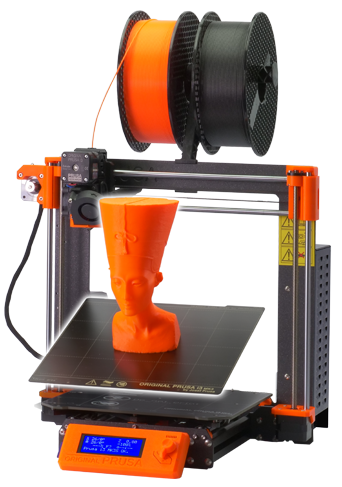
\includegraphics[scale=0.5]{figures/MK3s-home-new}}
        \caption{Image of the Prusa MK3s FDM 3D-Printer}
        \begin{quote}
            "Any sufficiently advanced technology is indistinguishable from magic."
            \begin{flushright}
                \tiny{--- Arthur C. Clarke}
            \end{flushright}
        \end{quote}
    \end{figure}

    \mysubsection{The technology}
    3D-Printing is a relative new technology which allows production of computer-designed three-dimensional models
    in certain materials.
    There are many different methods of 3D-Printing, but the far most common for home use is \textit{Fused filament
    fabrication} (FFF), or more commonly known as the trademarked term \textit{Fused deposition modeling} (FDM),
    which is the type used in this project.
    \\\\
    FDM stands for Filament-deposition-modeling;
    a method which extrudes thin strings of thermoplastic filament
    in layers as thin as 0.05mm and up to 1mm, controlled by computer numeric control (CNC) code.
    This allows the creation of models with great detail at a low cost, with the accuracy of stepper-motors.
    It also allows to re-use the commands and produce almost exact replicas of the same digital objects with
    little to no extra work.
    \\\\
    Unfortunately this 3D-Printing process is tedious, and can take several hours or even days.
    Since 3D-Printers are CNC machines, the FDM process is only a one way communication between the controller
    and the stepper motors.
    Meaning that during the process there exist little to no feedback from sensors for the result, while there are countless
    factors that play a role for the product from a single print operation.
    While printing any model, small errors that go undetected can be detrimental and require human intervention.
    Some failures can even cause harm to the machine itself, and has caused fires due to the high temperatures involved in
    the process.
    \\\\
    Luckily the technology is getting better, and more sensors are being added.
    This may include sensors for filament-runout to prevent printing without filament, or collision detection which detects
    if any motor meets resistance preventing damage to itself or humans.
    Alas it is still recommended that you stand by the machine for the entirety of the print, but people still leave their
    homes with the dishwasher running.

    \mysubsection{Continuous innovation}
    Computer technology is constantly moving forward, and 3D-Printing is no exception.
    Updates are rolling out continuously for all the different systems, some updates even fix third
    party integration problems.
    \\\\
    What really changes 3D-Printer updates is the possibility of sending digital physical upgrades, which you can print
    and change yourself.
    This enables larger beta-testing, cheaper and faster physical upgrading, and shorter production testing before a unit can ship.
    \\\\
    During this project the development-printer has received
    \begin{itemize}
        \item 2 physical updates
        \item 1 physical major version upgrade, requiring some new manufacturer parts
        \item 2 personal modifications for the project
        \item 5 software updates (and 1 personally compiled pre-release to fix project issue) \mycitation{prusa:github:versions}
    \end{itemize}

    \newpage

    \mysection{Terminology}
    \mysubsection{Printer parts}
    \begin{itemize}
        \item Extruder: The heated part of the printer which melts the plastic and extrudes it.
        \item Heatbed/printbed: The plate on which a print begins, often heated for better adhesion.
        Also comes in different materials like glass or PEI .
        \item Einsy/motherboard: The main electrical board of the printer which everything is connected to.
        \item Filament: The name of the material used to create models, in a continuous string on a spool.
        Usually made of either plastic or nylon, the most common types are PLA, ABS, PET-G, TPU, and PA-12 which holds
        their unique properties, print-settings, and prices.
        The filament is also what decides the color of the print, and color-pigments might change some properties too.
        \item MMU: Multi-material-upgrade, expansion for the 3D-Printer which allows the use of multiple filaments and
        changing of color during printing.
    \end{itemize}

    \mysubsection{Technical}
    \begin{itemize}
        \item Mesh: A digital file format method for 3d-objects.
        \item STL/OBJ: The some of the most used digital file formats for the mesh method.
        \item GCODE: The name of the instructions given to the 3D-Printer and \; is comments.
        These codes refer to single operations eg. \textit{M104 S215 \; set extruder temp}.
        GCODE might also refer to GCODE-file.
        \item GCODE-file: A file containing up to several hundred-thousand lines of GCODE commands.
        Usually one file per print-job.
        \item Slice: The operation where a digital mesh is processed to GCODE instructions that will replicate said object.
        This also handles settings like temperatures and speeds.
        \item Slicer: A program/application that does the slicing operation.
        Usually holds default settings for your printer, and some are proprietary.
    \end{itemize}
    \mycitation{reprap:gcode}

    \newpage

    \mysection{Technologies}
    \mysubsection{Octoprint}
    As of now, many 3D-Printers are open-source, which allows users to create their own tools and better the control they have.
    One such tool is \textit{Octoprint}, which runs on a raspberry-Pi, hosting a web interface for your 3D-Printer.
    \\\\
    The Octoprint server allows the user to read live sensor data from a web-interface, connect a camera, and even add plugins
    for more advanced control.
    Allowing such an expansion can ease large manufacturing by, e.g.
    , allowing the removal of a single part that has failed without having to stop the print loosing it entirely.
    \\\\
    Octoprint is tackling many common features requested by 3D-Printer companies, and hosting them available under the same
    service.
    This includes web-based automatic slicer, visualization of bed leveling, remote control of axis and temperature, and live camera streaming.
    All this works as both reliability and safety measures for a user, but 3D-Printing is still very complicated and requires
    training and experience for success.
    \\\\
    Octoprint has without a doubt added safety to printing, but is for now only available trough a web-browser,
    with little to no support for smaller screens without plugins.
    Luckily they have a REST-API available, which allow further development.
    Already there are multiple applications made for different mobile devices, but fewer are available for the wearable market.

    \mysubsection{Rest-API}
    \mysubsubsection{The technology}
    An application programming interface, is a gateway within an application designed for computer interactions.
    This allows any application to query the API and handle the answer as standardized formats.
    \\\\
    The REST or Restful only states that the host/server does not hold your state.
    The client therefore has to actively send all relevant information, but is in turn allowed to disseminate the entire
    application, and query only required information.
    \\\\
    Due to the stateless design there is no graph in which the application must be traversed, and even the api can call
    itself to make higher order functions.
    By design this can become an entirely new kind of application spaghetti, with too many endpoints and circular
    references.

    \begin{quote}
        "It is no silver bullet, but a powerful tool."
        \begin{flushright}
            \tiny{--- Christoffer O. Hern\ae s, CDO. Sbanken}
        \end{flushright}
    \end{quote}

    \mysubsubsection{Exposing APIs}
    APIs can divide an application to smaller \textit{Single responsibility} endpoints, or separate
    backend from frontend.
    The most used parts of a service can often be made into APIs in order to remove code-replication within a business,
    and sometimes those APIs can be opened directly to the customers.
    This allows the users to develop any automated solution themselves, which we can see some larger businesses doing.
    \\\\
    In the fintech market we have seen several uses of APIs, especially since the PSD2 directive was added by the EU .
    A popular example is how many norwegian banks are allowing the importing of external accounts, and the import of the
    norwegian state student loan service \textit{L\aa nekassen} into Sbanken
    \mycitation{laanekassen:psd2:sbanken}
    \\\\
    Other (especially open-source) applications can expose the entire application as an API allowing users to contribute
    with new solutions, like Octoprint allowing users to develop applications even for other devices.
    This is crucial to develop the TizenPrint application.

    \newpage

    \mysection{Planing the application and infrastructure}
    \mysubsection{The setup}
    The 3D-Printer only support GCODE commands using mostly the NIST RS274NGC Interpreter.
    This requires GCODE to either be supplied trough a SD-card directly in the 3D-Printer or by a physical connection.
    This is where Octoprint is connected.
    Octoprint is running on a RaspberryPi 3B+ using the Raspbian-Lite OS, in a custom built casing on the printer.
    This creates a small computer with a physical connection, and since Octoprint is accessible trough the web-interface
    it acts like a wireless bridge.
    \mycitation{reprap:nist}
    \\\\
    Octoprint is running its own web-service and allows certain operations even if the printer is turned off.
    It also hosts an Application-protocol-interface which allows other applications to access and use octoprint as a
    service-point connecting to the printer.

    \mysubsection{Goals of application}
    The application should first of all aim to substitute an operator in using a 3D-Printer, by allowing for easier
    access to an interface, quick controls and main information like temperature-readings.
    Ideally it should also act as a small safety feature to keep an eye on a running printer from a distance, even though
    leaving any running CNC machine is discouraged.
    \\\\
    It is therefore essential to the minimum viable product (MVP), that the application is able to show a live
    video-stream of the printer, and read the different temperatures in real time with minimal delay.
    Control of axis is also a priority, as this is an essential tool while operating the machine before and after
    print-jobs.
    Lastly the application should hold an option to start prints, although neither upload nor perform a slicing
    operation as that would be illogical to do on such a small device.

    \newpage

    \mysubsection{Planned architecture}
    \begin{figure}[h!]
        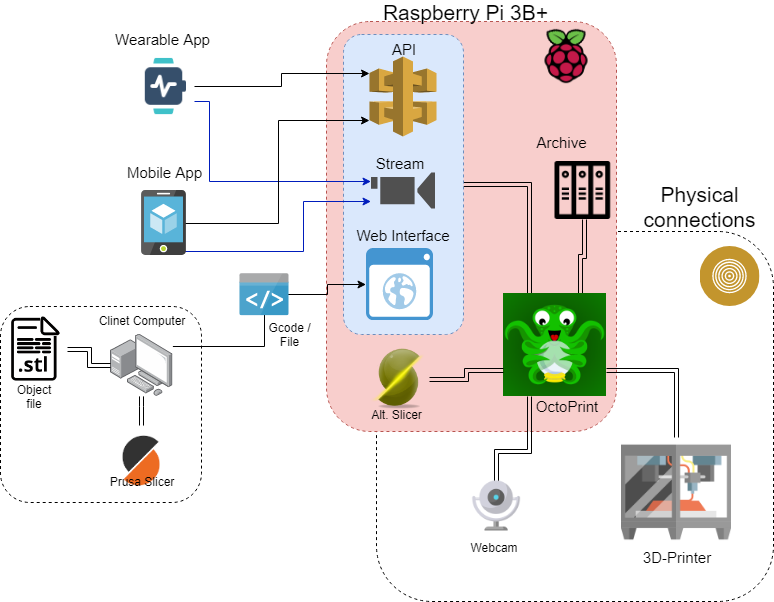
\includegraphics[scale=0.5]{figures/TizenPrint-architecture.png}
        \caption{Planned Architecture;
        With this setup the physical printer and webcam is isolated by physical
        connections from the rest of the world.}
    \end{figure}

    Octoprint is running as a service on a Raspberry Pi 3B+ (marked red), with access to its filesystem for storage and other
    external applications like an alternative slicer.
    Parts of octoprint needs to be exposed directly to the internet to act as a web-interface, these parts are marked as
    blue.
    \\\\
    Please note that the stream is available alone.
    This is due to the usual browser-implementation and makes development easier as it acts just like a still-image.
    This is what allows the stream to be accessed even though the rest of the application uses the API .
    \\\\
    Handheld and wearable devices are small in physical size.
    It is therefore not feasible to support all of Octoprints features on such devices.
    This is usually not a problem because such devices would typically be used mainly for monitoring and setting up printing,
    for which the full feature set is not needed.
    Meanwhile more complicated features like the setup of models can be done by a computer, where one normally would design
    the model anyways.
    Here we can slice the model to our preferred settings, and upload the gcode to octoprint where it will be stored on
    the raspberry pi filesystem.
    \\\\
    If wanted, the web-interface could also be ignored and the GCODE-file could be put directly on the 3D-Printers SD card
    manually.
    Octoprint is still able to read those files and start the printing-job operation on them.
    From a handheld or wearable device the ability to start a print-job is expected, as this allows a printer operator
    to use a computer away from the printer, and repeatedly start the same or a new job without having to slice again.

    \newpage

    \mysection{Development}
    \mysubsection{First looks}
    Development of the Tizen wearable watch application started by installing the tizen-studio.
    Tizen studio was not available to all operating systems even though it is built around Eclipse which is made in Java.
    Luckily there is still the ability to compile the source, and thus installing on the main development OS .
    \\\\
    The Tizen-studio gives a standard "Hello World" program, which worked in the simulator, but would not deploy to the
    physical device due to certificate requirement, which was not supported in the used OS .
    \\\\
    Unfortunately the only other available development computer running Windows 10 did not have a processor which met
    the requirements to run the emulator (Hyper-V compatible), nor was it placed in an environment which allowed the physical device to connect
    to wifi, thus not being able to deploy.
    The solution for deploy meant dual-booting into windows 10, and borrowing an external wifi-signal in another
    location, which alone accounted for major delays.

    \mysubsection{Choosing development language}
    Tizen-studio offers development as either a native application using C++/C or as a web-application running HTML/CSS/JS
    locally on the device.
    To try both\; a small dice-throwing application was developed, and it soon became clear that using the emulator to for
    each test took too long.
    Secondly the JavaScript language has easy to use built inn support for use of APIs, and would greatly increase the
    efficiency of testing as that could be done on the computer web-browser.
    Lastly the styling of the application was much easier to change due to a CSS supporting reusable definitions called
    classes.
    \\\\
    It is now also possible to develop in .NET C\# using Xamarin in microsoft visual studio.

    \mysubsection{Getting to know the tools}
    As an experiment, the simpler experimental application (MyPay) was developed in parallel.
    This application shows the balance on personal bank-accounts, and was later expanded to list and pay electronic invoices.
    \\\\
    During the development of said experiment-application, several issues were encountered.
    This included issues like the project settings needing to allow the use of external connections in order for the
    wearable-OS to allow the application to connect.
    \\\\
    This is where the issue of secrets arose.
    Since this application was to be hosted publicly on github, hosting private addresses and connection secrets for
    the API would allow others to gain unauthorized access.
    This would allow anyone to steal secrets and take control of the Octoprint-instance and the development 3D-Printer.
    To prevent this a file was made to hold said secrets, and excluded from git using gitignore, but with instructions in
    the project Readme.md

    \mysubsection{Inadequacy}
    Tizen-studio alone does not have many tools that assists development, and even some of the expected tools like the
    indention tool do little to nothing.
    Therefore, since TizenPrint is written in such a widely used web-languages (HTML/CSS/JS), it is possible to change
    the IDE .
    Since \textit{Jetbrains} has been the standard supplier of IDEs used in most courses, their product \textit{WebStorm} became the
    preferred tool.
    \\\\
    For fast testing and development;
    a visual result of the product being developed needs to be displayed after every change made.
    Since the TizenPrint application was written in the simple web-languages it was able to run from a browser.
    The web browser \textit{Google Chrome} has build inn development tools, and was selected for this projects mainly due to its
    ability to run JavaScript commands in a console and debug.
    \\\\
    While most browsers will display a square layout, the device holds a circular display.
    Even though the display is circular, the device uses the screen as square, and will place content outside the physical screen,
    not displaying anything.
    To expand the design, the background was set to a contrast color, and got a circular box over it to illustrate where
    the physical frame would be.

    \begin{figure}[h!]
        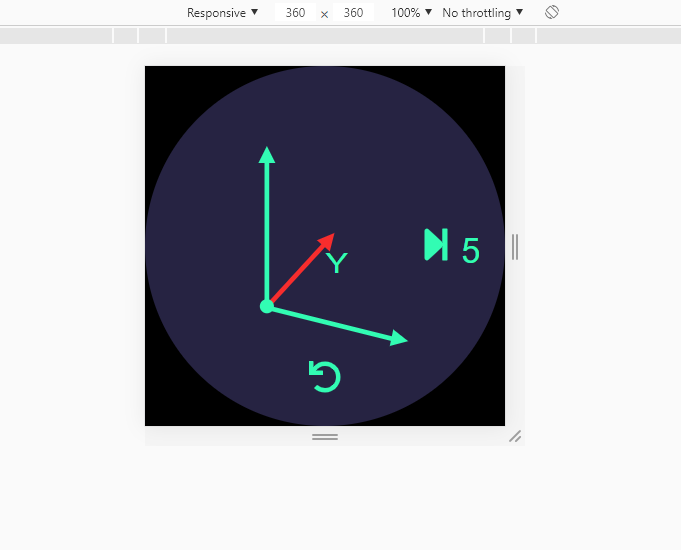
\includegraphics[scale=0.5]{figures/application-xyz-image.png}
        \caption{Screenshots of the application displayed in the \textit{Google Chrome} web browser.
        The black parts of the square will be placed outside the physical screen on the device.}
    \end{figure}

    \mysubsection{Security}
    \begin{itemize}
        \item Architecture / Endpoints
        \item Worst case misuse
        \item API key
        \item TLS / HTTPS
    \end{itemize}

    \mysubsection{Development tools}
    During this project several different tools have been used.
    This is the complete list with a short description
    \begin{itemize}
        \item GIT: Version control tool used to track any changes in any documentation or source-code created
        \item Github: Version control provider needed to use GIT, which also holds extra tools for development and issue-tracking.
        As a bonus this is also where both Octoprint and Prusa-Firmware is hosted.
        \item Intellij WebStorm: An IDE for web development, also supports LaTeX with plugins.
        Main development studio due to all the tools it provides.
        \item Tizen IDE: The main development studio has to be used for certificate management, emulator, and device-management.
        \item Google-Chrome: The main browser used for development.
        \item Arduino build tools: Used to compile the firmware for the 3D-Printer
        \item Windows 10: Main development OS
        \item Arch-Linux: Secondary linux-distro development, test and deploy OS
        \item Raspbian: Light linux-distro OS needed to host octoprint and control the printer.
        \item Octoprint: A web-service to control open-source 3D-Printers with a web interface.
        Also holds the API and is the tool which will be developed towards.
    \end{itemize}

    \newpage

    \mysection{Design}
    \mysubsection{Circular display}
    Working with a circular display is a rather interesting concept.
    Due to the bevels not following a straight line, while the screen effectively is outside the frame, it does mess with
    the design and layout languages CSS and HTML .
    Tizen-studio does provide a small package called the Circular-helper.js which is meant to support developers by
    keeping elements inside the frame on the device.
    Still it is often easier to just use strict design and pixel measures.
    Such design is usually not viable in normal web-design due to all the different devices that can access a site, but
    due to the application only supporting one device that is not an issue.
    \\\\
    Another aspect of the circular design is that it allows for some innovative figures and designs.
    Even though such a circular construction limits an already small screen, it allows the design to break certain standards,
    and move objects closer to the center of the screen.
    This forces the look to become less structured, and applies a more natural feel to almost any design,
    while only displaying the most relevant information.
    \mycitation{samsung:developer:galaxy-watch:DesignPrinciples}
    \\\\
    The circular bevels therefore promotes the use of rounded scrollbars, single displayed items, and even bent text along
    the edges of the device.

    \mysubsection{One page application}
    The setup of Tizen web applications does not support more than one page.
    Unlike normal browser design where you link to different files on the server, tizen only loads the first page, and
    refuses to handle anchors (links) as expected.
    Instead tizen uses a provided JavaScript to display different pages.
    This is essentially done by adding and removing a style-class, where only the container with the class "ui-page-active"
    is displayed, together with a possible footer which is always displayed.
    \\\\
    One page application files tend to get rather large, and can slow down development.
    Sometimes trickery can be used to load other files by Iframes and so on, but this often does not have the intended effect.
    It therefore becomes essential to move all possible aspects outside of the HTML, like scripts and SVGs in their own
    files.

    \mysubsection{Attention span}
    Wearable devices like watches are made to only be glanced at, usually while moving.
    Most applications are therefore designed only to show the most relevant information to a user.
    It is therefore important to have the app show the relevant information fast, with few interactions.
    For even a bit more complex interactions a larger device would be a more appealing choice.
    A simple interface is therefore crucial for the printer control applications.

    \mysubsection{Small display}
    The samsung galaxy watch has a display with high resolution, but in design it holds effectively 360 x 360 pixels,
    which is really small, only about a fifth of a normal computer screen.
    This limits the size of any text being displayed, and requires a lot of innovative design.
    \\\\
    One solution to this has been the usage of icons instead of text.
    This allows a much more efficient design for menus or footers, leaving a lot more space for the main content on the
    page.
    \\\\
    Another solution is to implement popper usage of the physical input from the device.
    The physical devise does have 2 buttons, and a rotating bevel, though only one of the buttons allows
    for change.
    This adds easier to reach tactile buttons with a response to the user, but testing of these inputs does require an
    emulator, which slows down development.
    Also, the expected functionality of the physical inputs needs to be apprised for the user.

    \mysubsection{The problem of icons}
    Regrettably icons is not a fix-all solution for small displays, and does come at its own cost.
    Even though most feel like icons does help with explaining the expected behaviour or meaning, they should only be used
    to assist the explanation with a text.
    This is due to the many icons being used not necessarily being standardised, or the illustrated object unknown to a
    potential user.
    \\\\
    A great example of icons not being recognised is the usage of the save-icon.
    The icon usually represents an old floppy-disk, which newer generations might never have experienced.
    This in turn makes the icon something we have to learn to recognise, and once learned it greatly increases the time
    it takes to find it, or associate the functionality of an interface.
    \\\\
    An argument of statistics therefore goes against the practice of icons, as they might be misinterpreted.
    If each icon holds a probability for misunderstanding, then each icon added will greatly increase the chance
    for at least one icon being misunderstood for each user.

    \mysubsection{Wearable device}
    As the intended device is a wearable watch, it is expected to be small in size.
    This physical limitation does also limit the size of internal components greatly, and then heat-dissipation even more.
    Such devices can therefore not hold powerful components, nor large batteries.
    Many other devices (e.g., the apple watch), limits the thread requirements of their applications to prevent bad
    development to impact the battery life of their device.
    \\\\
    Tizen OS does not set any such visible limits, and it is therefore recommended to limit background processes, and hard
    operations.
    In the development of this app this was discovered when a stream was added.
    Due to the single-page design of the application the stream was updated continuously, as long as the app was open,
    even if it was only showing temperatures.
    This lead to major decrease in battery-levels after only a few minutes of testing.
    \\\\
    The solution to both aforementioned usage-problems was simply to load/unload the stream, loading it only when it was
    required.

    \mysubsection{Accessibility}
    \centerline{
\includegraphics[scale=0.5]{figures/hoved_engelsk_farge_positiv.jpg}}
    \mysubsubsection{Legal requirements}
    Another major issue unveiled during development is the lack of integrated accessibility features.
    In Norway developers are strongly regulated by the EU and Norwegian laws, requiring developers to implement accessibility
    features to their applications.
    This includes (but is not limited to) things like, blind users, deaf users, or users otherwise unable to use the
    provided interface like amputees.
    \\\\
    This project will not focus too much on accessibility, as it is not meant to be published nor profitable.
    Nevertheless it is important to mention the severity of the inadequacy for accessibility features in the Tizen OS,
    and some of what would have to be done in the case of publishing and profiting.

    \mysubsubsection{DIFI standards}
    DIFI translated is (Agency for Public Management and eGovernment).
    As an organization they handle many parts for human prosperity, and includes many different topics.
    \mycitation{difi:about}
    \\\\
    What is relevant here is the sub-part for accessibility, which difi has an entire sub-domain for.
    This includes requirements like minimum icon or text size, requirements for the readability
    of the fonts, help for screen-readers and much more.
    \mycitation{difi:uu}
    \\\\
    Now Tizen OS does offer a lot of build inn accessibility features, but is overly complicated to implement into a new
    application.
    The consequence of this is that few available applications implements screen readers,an can not be used with a screen reader.
    This is especially problematic, as screen readers can usually manage to browse most features and web pages even though it is not
    implemented directly.

    %Tving alltid til ny side
    \newpage
    %Laster inn referanser
    \bibliography{citation-db}
    %Legg inn i contents (toc)
    \addcontentsline{toc}{section}{References}

\end{document}